\documentclass[11pt,a4paper]{article}

\usepackage[utf8]{inputenc}
\usepackage[margin=0.85in]{geometry}
\usepackage{amsmath,amssymb}
\usepackage{booktabs}
\usepackage{tabularx}
\usepackage{graphicx}
\usepackage{hyperref}
\usepackage{enumitem}
\usepackage{listings}
\usepackage{xcolor}

\hypersetup{
    colorlinks=true,
    linkcolor=blue!75!black,
    urlcolor=blue!75!black
}

\setlist[itemize]{noitemsep, topsep=2pt}
\setlist[enumerate]{noitemsep, topsep=2pt}

\lstset{
    basicstyle=\ttfamily\footnotesize,
    breaklines=true,
    frame=single,
    backgroundcolor=\color{gray!8},
    rulecolor=\color{gray!30},
    keywordstyle=\color{blue!80!black}\bfseries,
    commentstyle=\color{green!50!black}\itshape,
    stringstyle=\color{red!60!black},
    numbers=none
}

\title{\textbf{ESP32 Digital Signature Benchmark}\\[0.2em]\large Phase B: Integrated Network Handshake Benchmark (Over Real Wi-Fi)\\[0.2em]\normalsize FYP Documentation: Embedded VPN Client}
\author{Department of Computer Engineering}
\date{October 2026}

\begin{document}

\maketitle

\section{Phase B Overview: Live Network Handshake Benchmark}

While Phase A evaluated raw cryptographic operations directly in ESP32 chip memory, Phase B evaluates the full 3-way mutual authentication handshake executed over real local Wi-Fi and TCP sockets connecting an ESP32 client to a laptop gateway server.

This benchmark captures real-world embedded network characteristics:
\begin{itemize}
    \item TCP socket transport delays over IEEE 802.11 b/g/n wireless connections.
    \item End-to-end handshake latency including message transmission, signature generation, and verification on both sides.
    \item Over-the-air byte footprint and its impact on radio transmission stability.
    \item Latency predictability and jitter across multiple consecutive connection attempts.
\end{itemize}

Three cryptographic algorithms were benchmarked under identical network conditions:
\begin{enumerate}
    \item \textbf{Ed25519:} Twisted Edwards Curve25519 with Libsodium on the ESP32 and Python cryptography on the server.
    \item \textbf{ECDSA P-256:} NIST prime curve secp256r1 with ESP32 mbedTLS and Python cryptography.
    \item \textbf{RSA-3072:} Classical 3072-bit RSA with PKCS\#1 v1.5 padding and SHA-256 at an equivalent 128-bit security level.
\end{enumerate}

\section{Key Performance Indicators (KPIs)}

The Phase B evaluation profiles five network and system performance metrics:

\begin{itemize}
    \item \textbf{NET-1 (Total Handshake Latency):} Total elapsed time in milliseconds from the transmission of the initial server challenge to the completion of mutual verification on both ends.
    \item \textbf{NET-2 (Wire Overhead per Handshake):} The exact number of bytes exchanged across the TCP socket during the 3-way authentication sequence (Message 1 + Message 2 + Message 3).
    \item \textbf{NET-3 (Handshake Success Rate):} The percentage of initiated handshakes that successfully verified digital signatures without timing out or dropping packets.
    \item \textbf{NET-4 (Latency Jitter / Standard Deviation):} The variability in handshake duration across consecutive runs, indicating connection predictability.
    \item \textbf{NET-5 (Radio Channel Occupancy):} Qualitative impact of packet size on channel airtime and battery efficiency.
\end{itemize}

\begin{table}[htbp]
\centering
\small
\caption{Summary of Phase B Benchmarking KPIs}
\label{tab:phase_b_kpis}
\begin{tabularx}{\textwidth}{ll X}
\toprule
\textbf{KPI ID} & \textbf{Metric Name} & \textbf{Operational Significance} \\
\midrule
NET-1 & Total Handshake Latency & Real-world connection setup delay experienced by the IoT device \\
NET-2 & Total Wire Payload & Volume of TCP authentication traffic transmitted over the radio \\
NET-3 & Success Rate & Reliability of handshake completion under real network conditions \\
NET-4 & Latency Standard Deviation & Stability and absence of latency spikes across consecutive connections \\
NET-5 & Radio On-Time & Energy overhead determined by the byte size of transmitted packets \\
\bottomrule
\end{tabularx}
\end{table}

\section{Benchmark Results and Comparison}

\subsection{Performance Summary}

Table \ref{tab:comparison_summary} presents the empirical results measured across all test runs on the live local network (ESP32 IP: \texttt{10.27.228.175}, Laptop IP: \texttt{10.27.228.216} on TCP Port 9000).

\begin{table}[htbp]
\centering
\caption{Phase B Network Handshake Benchmark Results Comparison}
\label{tab:comparison_summary}
\begin{tabular}{l c c c c c}
\toprule
\textbf{Algorithm} & \textbf{Runs} & \textbf{Avg Latency (ms)} & \textbf{Min Latency} & \textbf{Max Latency} & \textbf{Wire Payload} \\
\midrule
\textbf{Ed25519}     & \textbf{20} & \textbf{249.48 ms} & \textbf{238.71 ms} & \textbf{260.79 ms} & \textbf{198 Bytes} \\
\textbf{ECDSA P-256} & 20          & 737.01 ms          & 267.49 ms          & 1,009.39 ms        & 212 Bytes \\
\textbf{RSA-3072}    & 10          & 750.90 ms          & 501.63 ms          & 1,112.68 ms        & 838 Bytes \\
\bottomrule
\end{tabular}
\end{table}

\subsection{Detailed Run-by-Run Iteration Records}

Tables \ref{tab:ed25519_runs}, \ref{tab:ecdsa_runs}, and \ref{tab:rsa_runs} document the individual timing measurements recorded for every handshake run.

\begin{table}[htbp]
\centering
\footnotesize
\caption{Ed25519 Handshake Latency across 20 Consecutive Iterations (Mean = 249.48 ms, StdDev = 5.28 ms)}
\label{tab:ed25519_runs}
\begin{tabular}{lcccccccccc}
\toprule
\textbf{Run} & \textbf{\#1} & \textbf{\#2} & \textbf{\#3} & \textbf{\#4} & \textbf{\#5} & \textbf{\#6} & \textbf{\#7} & \textbf{\#8} & \textbf{\#9} & \textbf{\#10} \\
Latency (ms) & 245.34 & 240.82 & 250.74 & 251.27 & 252.33 & 248.57 & 238.71 & 251.91 & 254.27 & 246.89 \\
\midrule
\textbf{Run} & \textbf{\#11} & \textbf{\#12} & \textbf{\#13} & \textbf{\#14} & \textbf{\#15} & \textbf{\#16} & \textbf{\#17} & \textbf{\#18} & \textbf{\#19} & \textbf{\#20} \\
Latency (ms) & 256.03 & 248.18 & 250.08 & 256.25 & 247.22 & 241.64 & 247.90 & 251.18 & 249.53 & 260.79 \\
\bottomrule
\end{tabular}
\end{table}

\begin{table}[htbp]
\centering
\footnotesize
\caption{ECDSA P-256 Handshake Latency across 20 Consecutive Iterations (Mean = 737.01 ms, StdDev = 207.15 ms)}
\label{tab:ecdsa_runs}
\begin{tabular}{lcccccccccc}
\toprule
\textbf{Run} & \textbf{\#1} & \textbf{\#2} & \textbf{\#3} & \textbf{\#4} & \textbf{\#5} & \textbf{\#6} & \textbf{\#7} & \textbf{\#8} & \textbf{\#9} & \textbf{\#10} \\
Latency (ms) & 267.49 & 586.41 & 584.52 & 581.71 & 589.46 & 590.61 & 585.09 & 924.02 & 757.03 & 1000.98 \\
\midrule
\textbf{Run} & \textbf{\#11} & \textbf{\#12} & \textbf{\#13} & \textbf{\#14} & \textbf{\#15} & \textbf{\#16} & \textbf{\#17} & \textbf{\#18} & \textbf{\#19} & \textbf{\#20} \\
Latency (ms) & 1004.97 & 1009.39 & 694.63 & 912.86 & 965.30 & 584.17 & 849.89 & 818.23 & 585.33 & 848.17 \\
\bottomrule
\end{tabular}
\end{table}

\begin{table}[htbp]
\centering
\footnotesize
\caption{RSA-3072 Handshake Latency across 10 Iterations (Mean = 750.90 ms, StdDev = 191.43 ms)}
\label{tab:rsa_runs}
\begin{tabular}{lcccccccccc}
\toprule
\textbf{Run} & \textbf{\#1} & \textbf{\#2} & \textbf{\#3} & \textbf{\#4} & \textbf{\#5} & \textbf{\#6} & \textbf{\#7} & \textbf{\#8} & \textbf{\#9} & \textbf{\#10} \\
Latency (ms) & 1112.68 & 643.05 & 501.63 & 718.55 & 756.65 & 523.85 & 553.45 & 908.08 & 1005.34 & 785.73 \\
\bottomrule
\end{tabular}
\end{table}

\section{Selection Rationale for Ed25519 on Live Networks}

The live Wi-Fi measurements provide empirical validation for selecting Ed25519 for the embedded IoT VPN client:

\begin{enumerate}
    \item \textbf{Three-Fold Latency Advantage (249.48 ms vs. 737.01 ms / 750.90 ms):}  
    Ed25519 completed mutual authentication handshakes in an average of 249.48 ms. Both ECDSA and RSA required roughly 740 to 750 ms, making Ed25519 approximately $3\times$ faster. In battery-powered IoT systems that wake up, connect, transmit sensor data, and sleep, this directly cuts active radio duration by 66\%.

    \item \textbf{Minimal Latency Jitter (Standard Deviation of 5.28 ms):}  
    Ed25519 demonstrated remarkable timing consistency, ranging tightly between 238.71 ms and 260.79 ms ($\sigma = 5.28\text{ ms}$). In contrast, ECDSA ranged from 267.49 ms to 1,009.39 ms ($\sigma = 207.15\text{ ms}$), and RSA ranged from 501.63 ms to 1,112.68 ms ($\sigma = 191.43\text{ ms}$). Ed25519 ensures deterministic connection scheduling without latency spikes.

    \item \textbf{Four-Fold Smaller Transmission Payload (198 Bytes vs. 838 Bytes):}  
    Total authentication traffic for Ed25519 was only 198 bytes across all 3 handshake messages. RSA required 838 bytes ($4.2\times$ larger). The compact frame size prevents packet fragmentation, fits comfortably within standard 802.11 MTUs, and minimizes airtime contention in dense sensor deployments.
\end{enumerate}

\section{Live Terminal Output Verification}

The terminal captures below record the benchmark server outputs during live hardware execution:

\subsection{Ed25519 Execution Output}

Figure \ref{fig:term_ed25519} shows the server logs for all 20 Ed25519 runs, with consistent ~250 ms completion times and zero packet dropouts.

\begin{figure}[htbp]
\centering
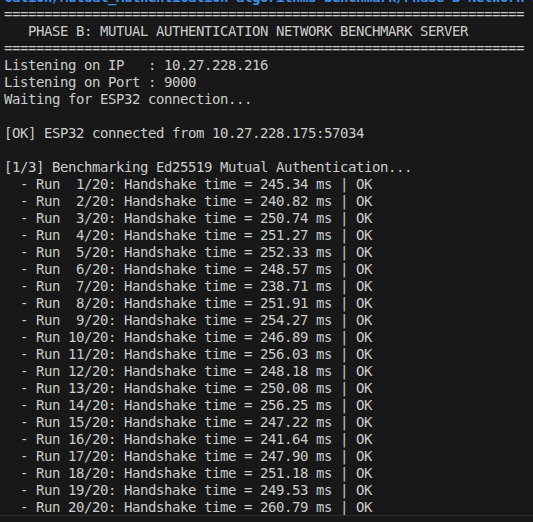
\includegraphics[width=0.72\textwidth]{screenshots/terminal_ed25519.png}
\caption{Gateway server terminal capture: Ed25519 benchmark (20/20 runs successful).}
\label{fig:term_ed25519}
\end{figure}

\subsection{ECDSA P-256 Execution Output}

Figure \ref{fig:term_ecdsa} displays the 20 ECDSA runs, showing latency fluctuations between 267 ms and 1,009 ms.

\begin{figure}[htbp]
\centering
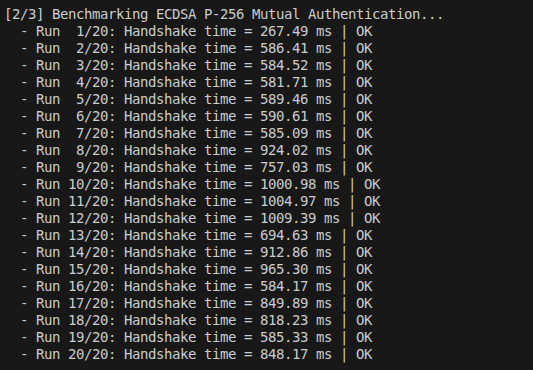
\includegraphics[width=0.72\textwidth]{screenshots/terminal_ecdsa.png}
\caption{Gateway server terminal capture: ECDSA P-256 benchmark (20/20 runs successful).}
\label{fig:term_ecdsa}
\end{figure}

\subsection{RSA-3072 Execution Output}

Figure \ref{fig:term_rsa} displays the 10 RSA runs, illustrating the impact of 384-byte signature computations and transmissions.

\begin{figure}[htbp]
\centering
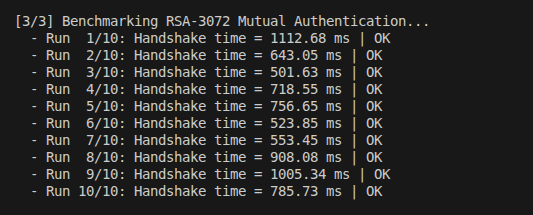
\includegraphics[width=0.72\textwidth]{screenshots/terminal_rsa.png}
\caption{Gateway server terminal capture: RSA-3072 benchmark (10/10 runs successful).}
\label{fig:term_rsa}
\end{figure}

\subsection{Final Comparison Table Output}

Figure \ref{fig:term_summary} displays the terminal output summarizing all tested algorithms.

\begin{figure}[htbp]
\centering
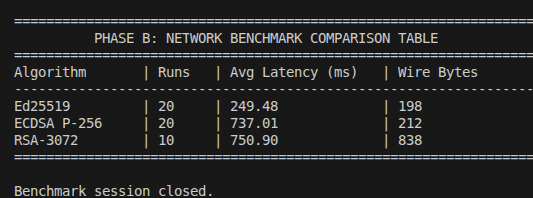
\includegraphics[width=0.72\textwidth]{screenshots/terminal_summary.png}
\caption{Gateway server terminal capture: Final comparison summary table.}
\label{fig:term_summary}
\end{figure}

\section{Graphical Benchmark Visualizations}

The figures below plot the empirical metrics across average latency, total wire bytes, and run-by-run stability:

\subsection{Handshake Latency Comparison}

Figure \ref{fig:plot_latency} compares the average handshake latency across algorithms, including standard deviation error bars.

\begin{figure}[htbp]
\centering
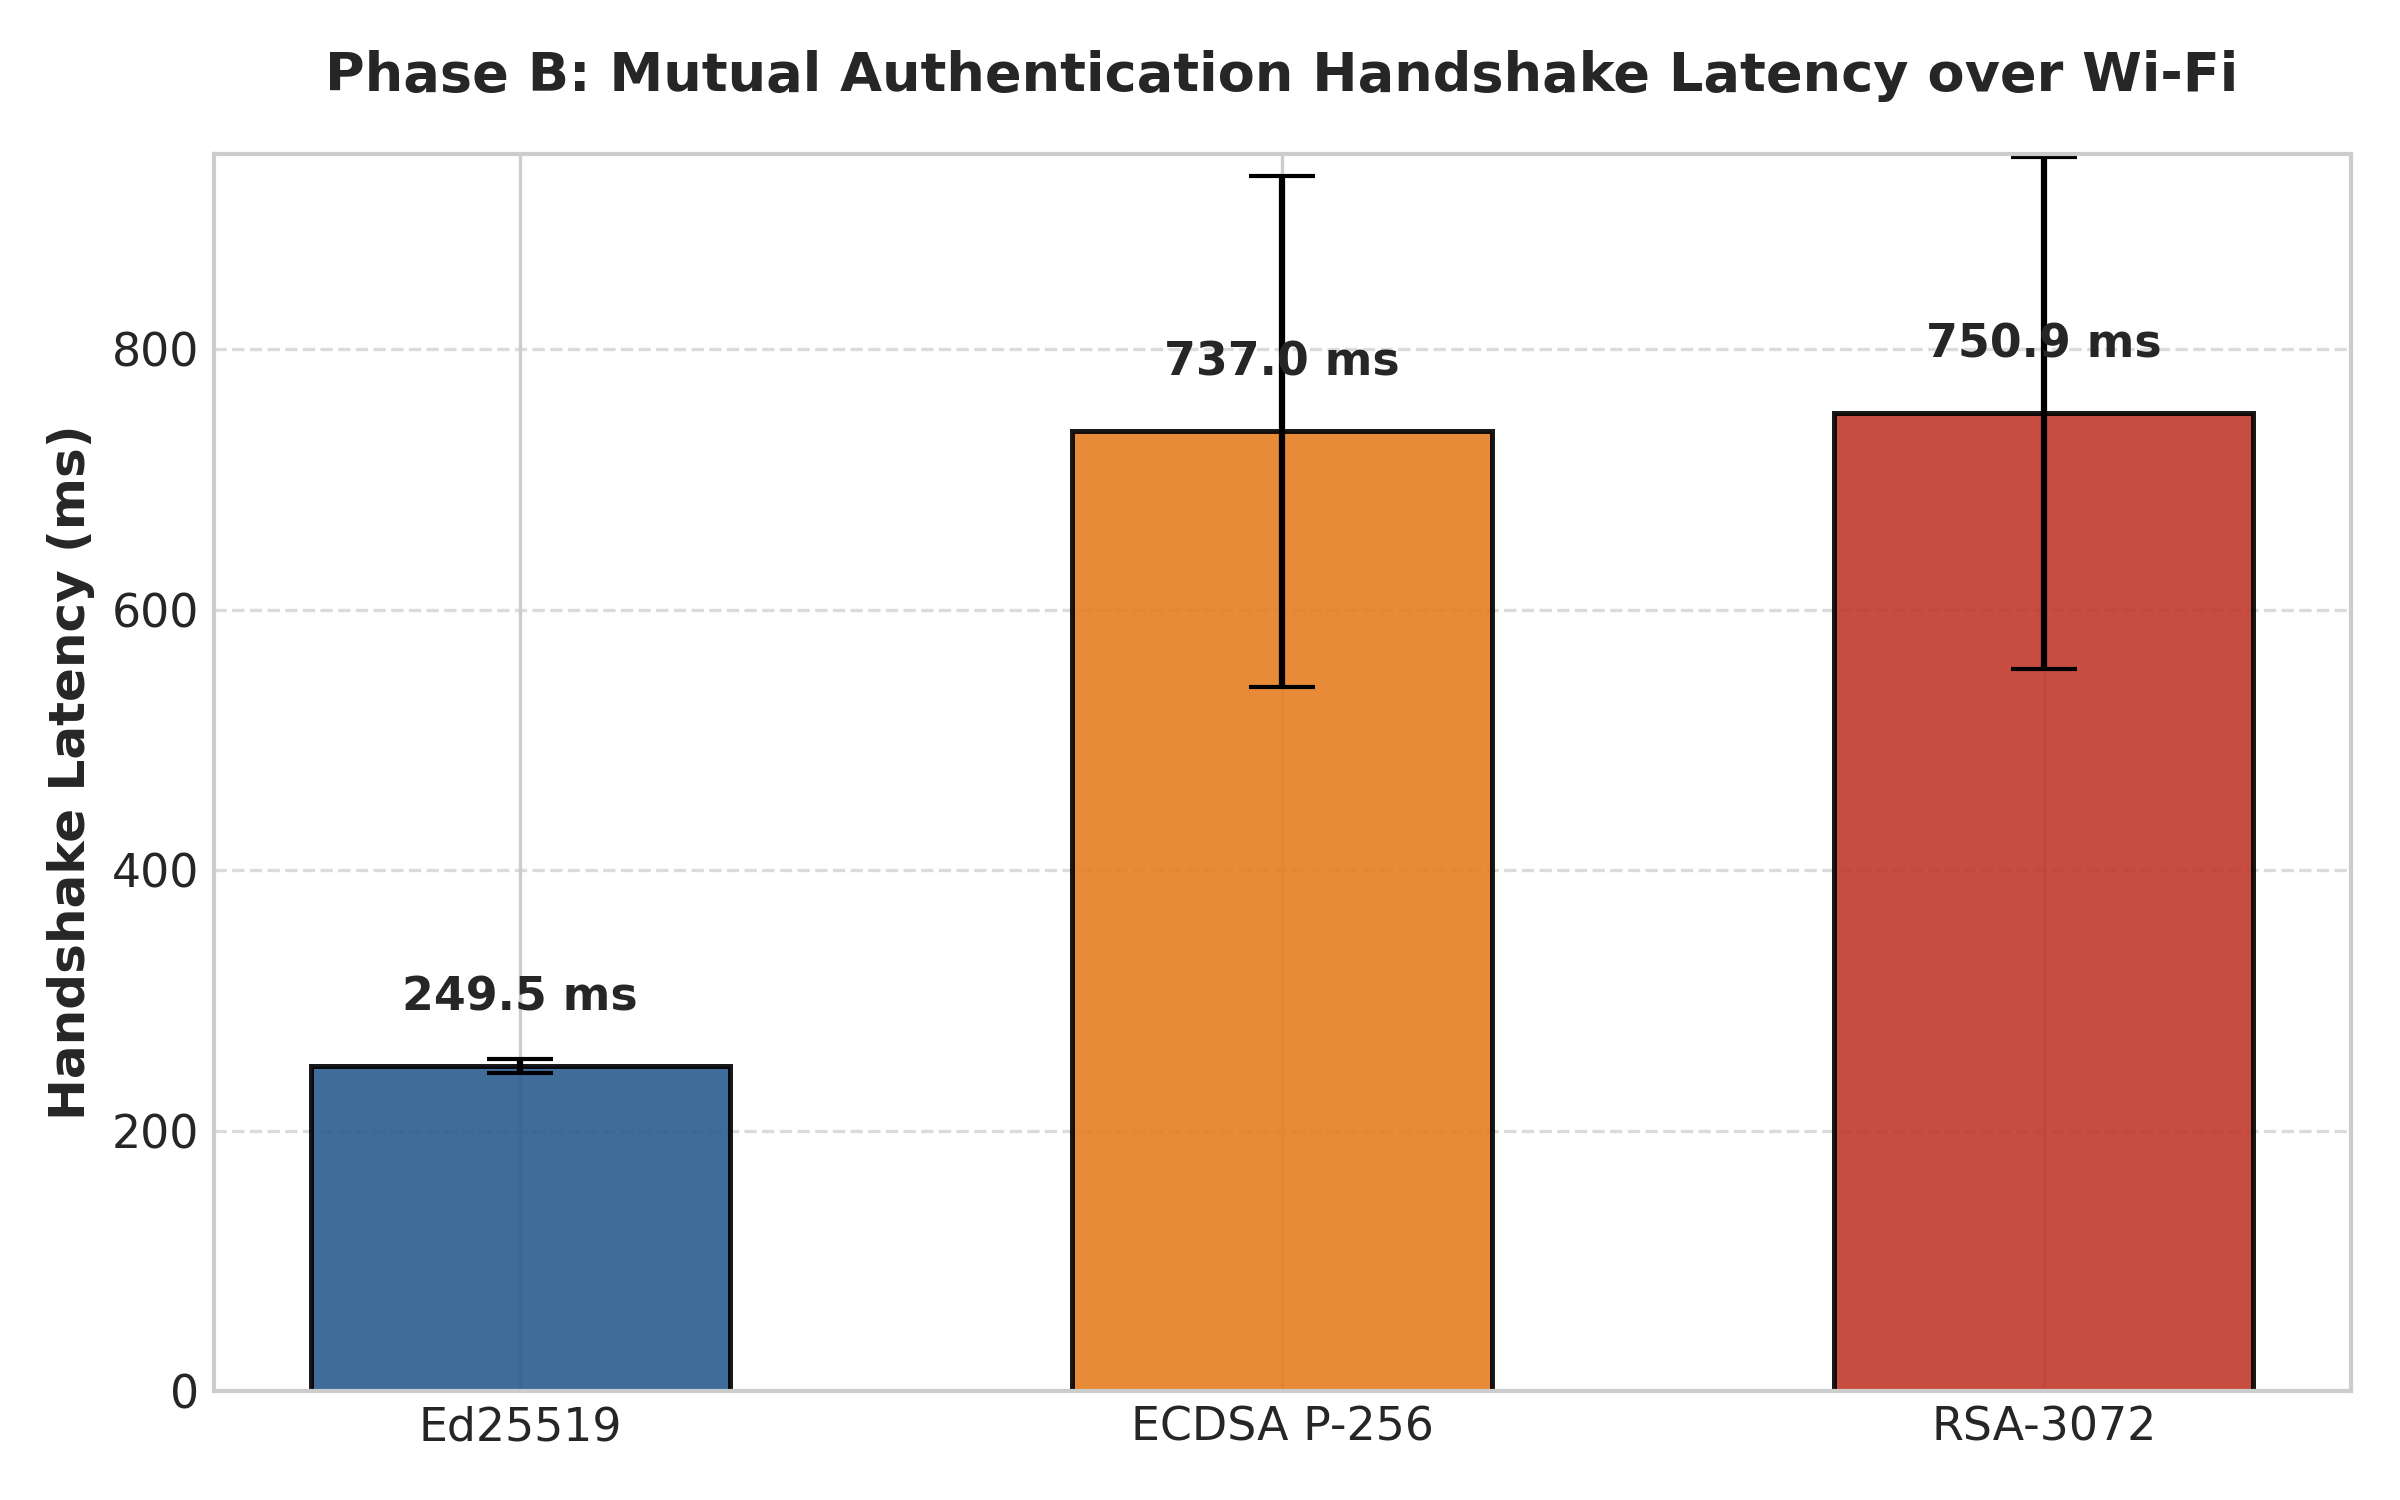
\includegraphics[width=0.75\textwidth]{graphs/fig_network_latency_comparison.png}
\caption{Average mutual authentication handshake latency over Wi-Fi (with standard deviation error bars).}
\label{fig:plot_latency}
\end{figure}

\subsection{Communication Wire Payload Overhead}

Figure \ref{fig:plot_wire} compares the total authentication payload exchanged over the TCP socket.

\begin{figure}[htbp]
\centering
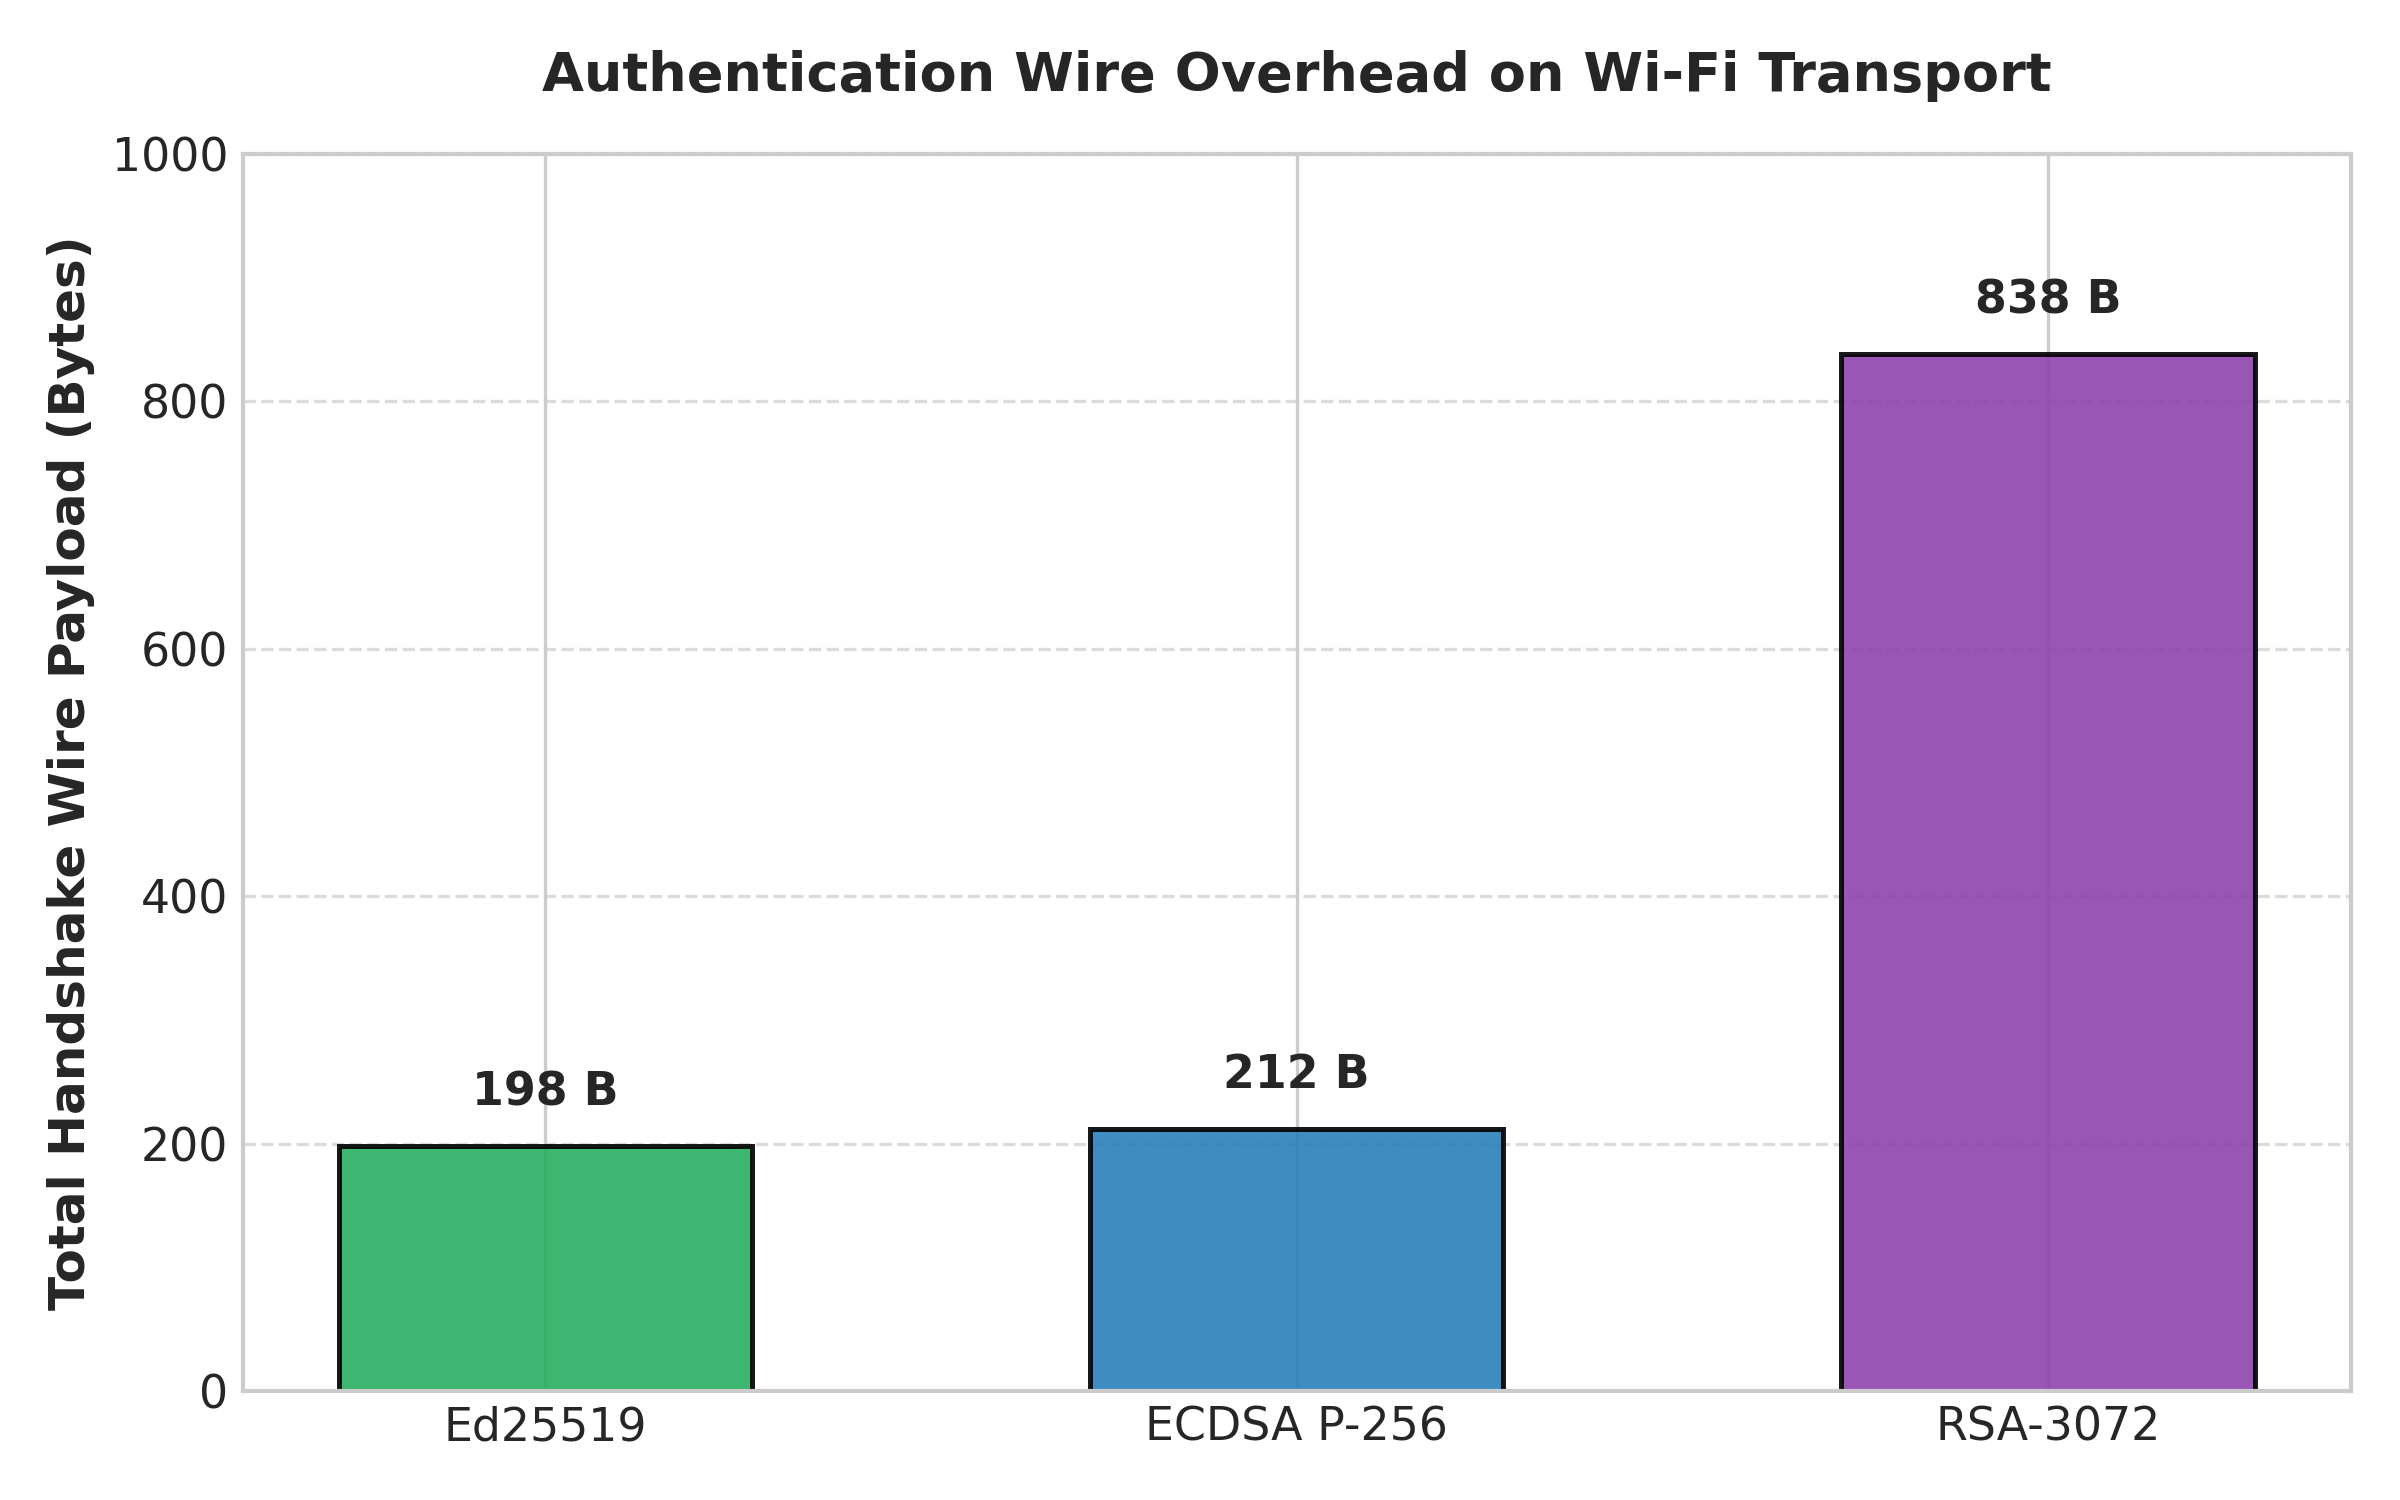
\includegraphics[width=0.75\textwidth]{graphs/fig_wire_overhead_comparison.png}
\caption{Total authentication handshake wire payload on Wi-Fi (Bytes per complete 3-way exchange).}
\label{fig:plot_wire}
\end{figure}

\subsection{Run-by-Run Latency Stability Distribution}

Figure \ref{fig:plot_distribution} illustrates the stability of each algorithm across consecutive runs. Ed25519 remains flat and predictable, while ECDSA and RSA show noticeable variance.

\begin{figure}[htbp]
\centering
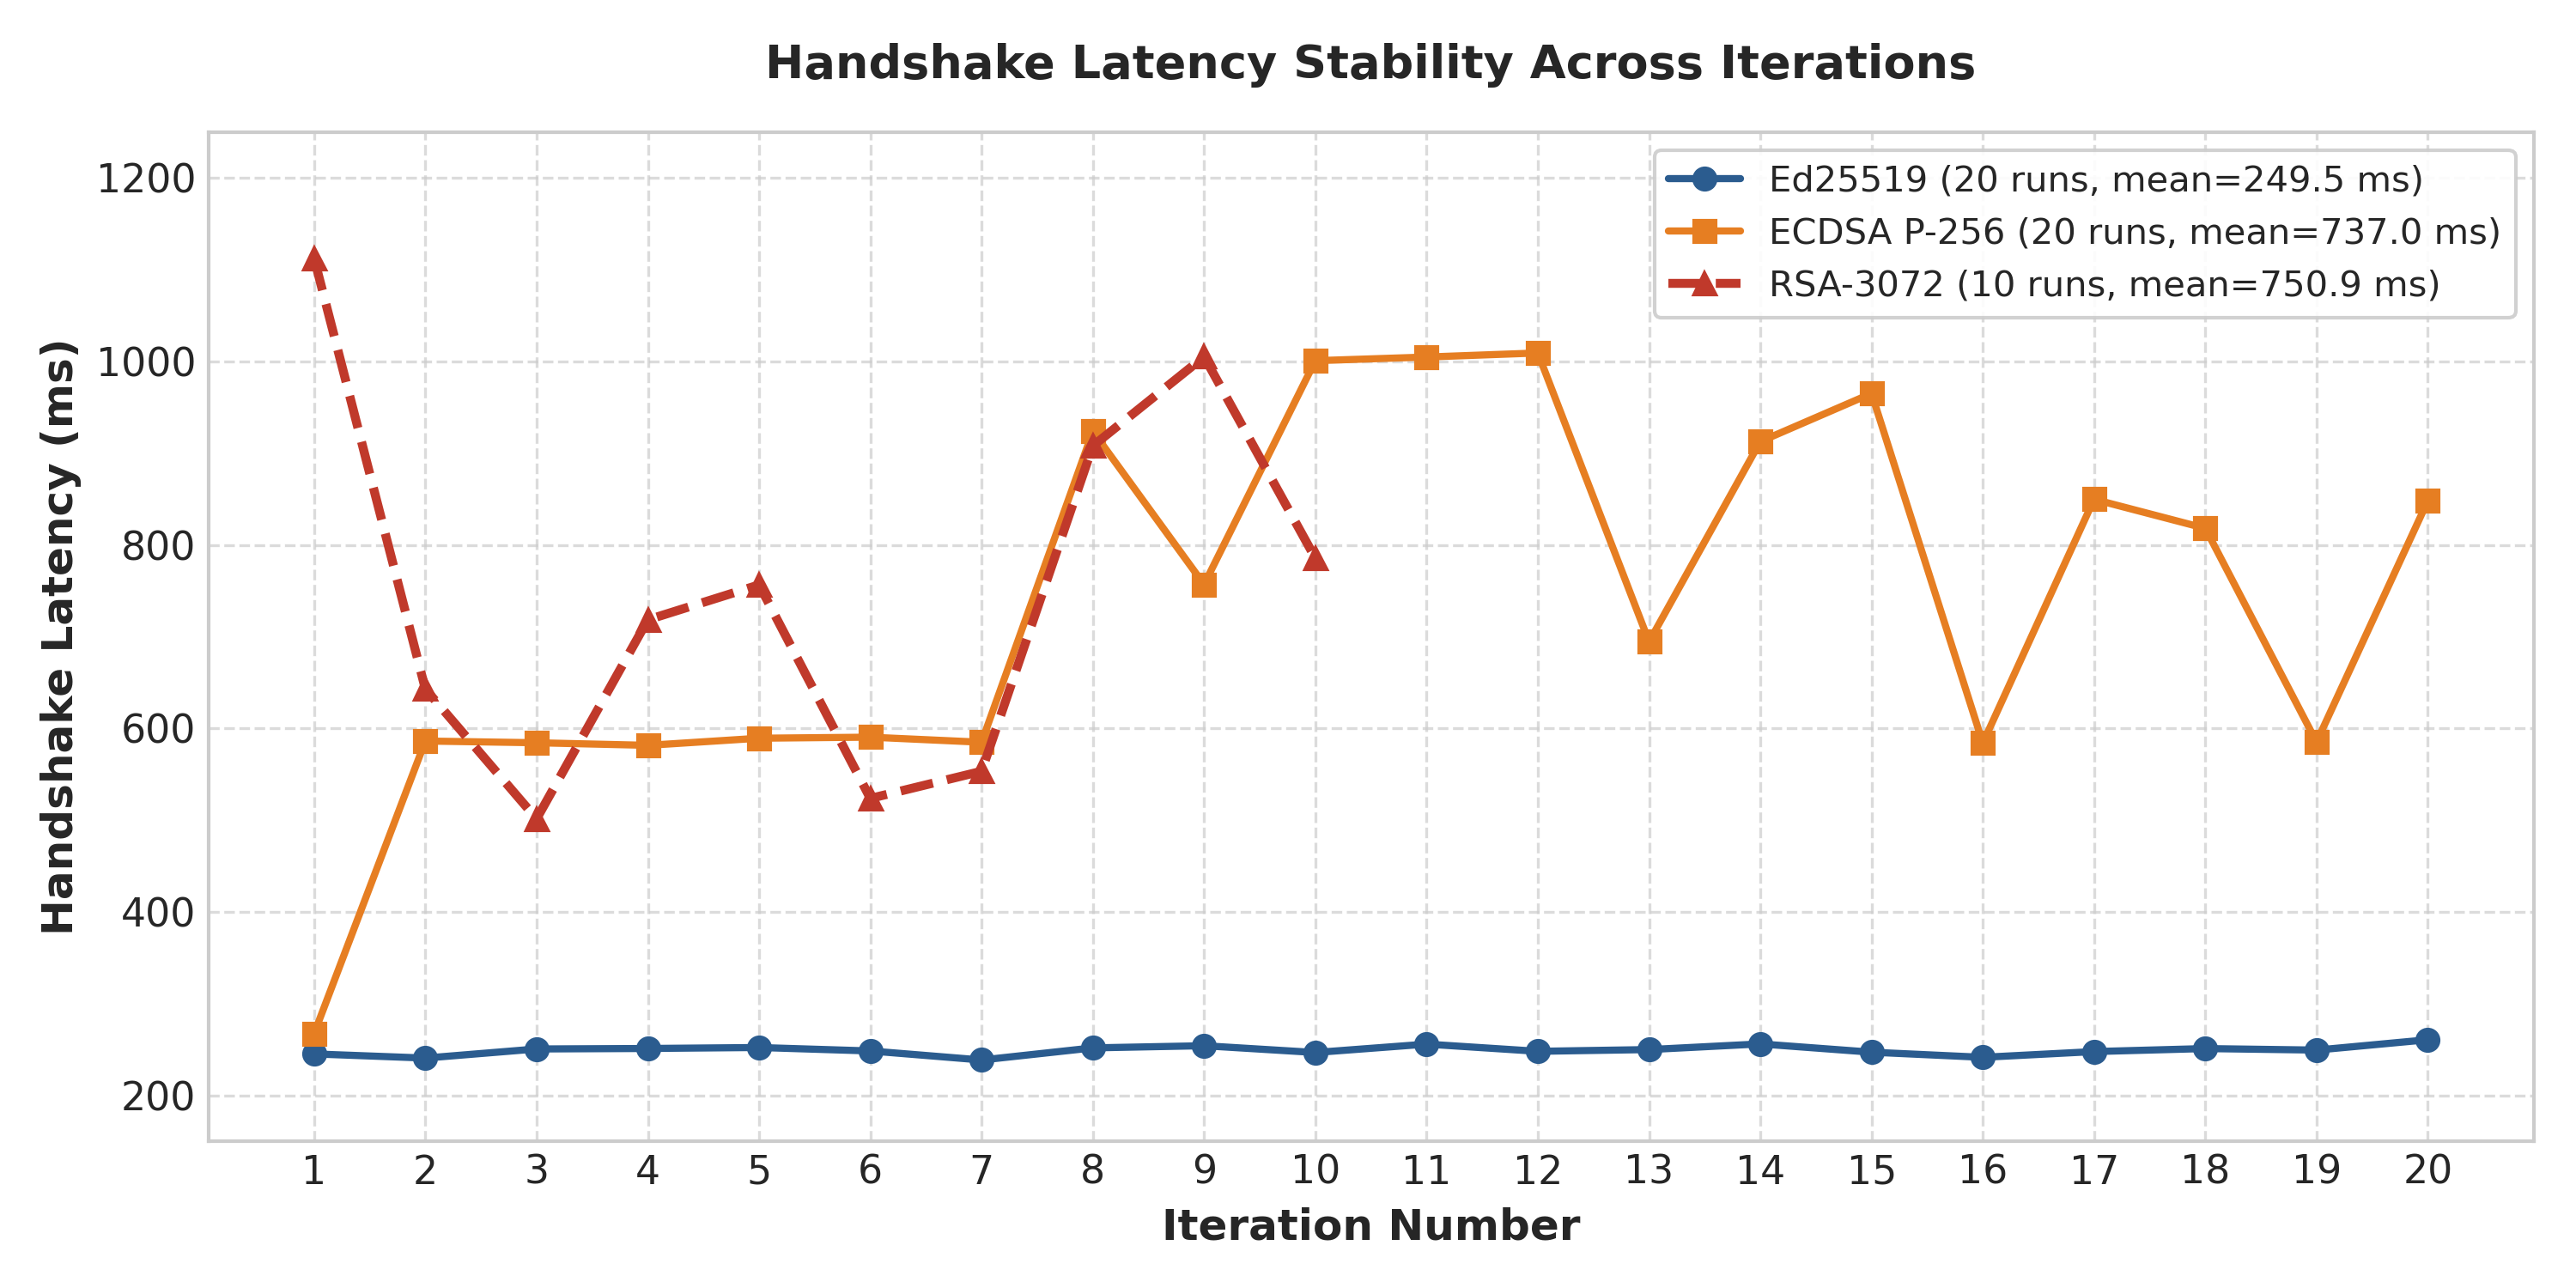
\includegraphics[width=0.88\textwidth]{graphs/fig_handshake_run_distribution.png}
\caption{Iteration-by-iteration latency comparison showing Ed25519 consistency vs. ECDSA/RSA volatility.}
\label{fig:plot_distribution}
\end{figure}

\section{Phase B Network Benchmark Algorithm and Pseudocode}

The Phase B benchmark profiles the complete network handshake across the ESP32 client and the Python gateway server. For each cryptographic algorithm (Ed25519, ECDSA P-256, and RSA-3072), the benchmark executes a series of live 3-way mutual authentication handshakes over a TCP/IP socket on a local Wi-Fi connection.

High-resolution hardware timers measure end-to-end handshake latency ($T_{\text{handshake}}$), client cryptographic computation time ($T_{\text{crypto}}$), network transit time ($T_{\text{net}} = T_{\text{handshake}} - T_{\text{crypto}}$), and wire byte counters. The complete benchmarking logic is shown below:

\begin{lstlisting}[language=Python, caption={Phase B Network Benchmark Algorithm and Execution Flow}]
# =========================================================================
# PHASE B NETWORK BENCHMARK: ORCHESTRATION & MEASUREMENT PSEUDOCODE
# =========================================================================

# Step 1: Benchmark Suite Configuration & Network Initialization
ALGORITHMS = [
    {"name": "Ed25519",     "id": 0x01, "runs": 20, "sig_bytes": 64},
    {"name": "ECDSA P-256", "id": 0x02, "runs": 20, "sig_bytes": 71},
    {"name": "RSA-3072",    "id": 0x03, "runs": 10, "sig_bytes": 384}
]

connect_wifi(SSID, PASSWORD)
socket = tcp_connect(GATEWAY_IP, PORT=9000)

all_benchmark_results = []

# Step 2: Iterate Across Each Cryptographic Benchmark
for algo in ALGORITHMS:
    print("Starting network benchmark for:", algo.name)
    
    # 2.1 Send command to server (Command ID + Run Count)
    send_tcp_packet(socket, payload=[algo.id, algo.runs])
    
    # 2.2 Exchange public identity keys (one-time setup)
    send_tcp_packet(socket, payload=client_public_key)
    server_public_key = recv_tcp_packet(socket)
    
    handshake_latencies = []
    crypto_latencies    = []
    network_latencies   = []
    total_wire_bytes    = 0
    
    # Step 3: Run-by-Run Network Handshake Benchmark Loop
    for run in range(1, algo.runs + 1):
        # --- Message 1: Server Challenge Nonce (Server -> ESP32) ---
        # Server generates 32-byte nonce and sends to client
        server_challenge = recv_tcp_packet(socket)     # 32 bytes
        t_handshake_start = get_timestamp_ms()
        
        # --- Message 2: ESP32 Processing & Response (ESP32 -> Server) ---
        t_crypto_start = get_timestamp_us()
        client_signature = crypto_sign(server_challenge, client_private_key)
        client_challenge = generate_random_bytes(32)
        t_sign_duration  = get_timestamp_us() - t_crypto_start
        
        # ESP32 transmits Signature + Challenge Nonce
        msg2_payload = client_signature + client_challenge
        send_tcp_packet(socket, payload=msg2_payload)
        
        # --- Message 3: Server Verification & Server Signature ---
        # Server verifies client signature against server_challenge
        # Server signs client_challenge with server_private_key
        # Server returns server_signature
        server_signature = recv_tcp_packet(socket)
        
        # --- Client Verification & Handshake Completion ---
        t_verify_start = get_timestamp_us()
        is_valid = crypto_verify(server_signature, client_challenge, server_public_key)
        t_verify_duration = get_timestamp_us() - t_verify_start
        assert is_valid == True, "Server signature verification failed!"
        
        t_handshake_end = get_timestamp_ms()
        
        # --- Step 4: Metric Calculation per Iteration ---
        run_handshake_ms = t_handshake_end - t_handshake_start
        run_crypto_ms    = (t_sign_duration + t_verify_duration) / 1000.0
        run_network_ms   = run_handshake_ms - run_crypto_ms
        
        # Wire bytes: 2-byte length header + payload for MSG1, MSG2, MSG3
        run_wire_bytes   = (2 + len(server_challenge)) + \
                           (2 + len(msg2_payload)) + \
                           (2 + len(server_signature))
        
        handshake_latencies.append(run_handshake_ms)
        crypto_latencies.append(run_crypto_ms)
        network_latencies.append(run_network_ms)
        total_wire_bytes += run_wire_bytes
        
        print(f"  Run {run}/{algo.runs}: Handshake = {run_handshake_ms:.2f} ms "
              f"(Crypto: {run_crypto_ms:.2f} ms, Net: {run_network_ms:.2f} ms) | OK")
    
    # Step 5: Statistical Aggregation across All Runs
    avg_handshake = mean(handshake_latencies)
    min_handshake = min(handshake_latencies)
    max_handshake = max(handshake_latencies)
    jitter_stddev = std_dev(handshake_latencies)
    avg_wire_size = total_wire_bytes / algo.runs
    
    all_benchmark_results.append({
        "algorithm": algo.name,
        "runs": algo.runs,
        "avg_latency_ms": avg_handshake,
        "min_latency_ms": min_handshake,
        "max_latency_ms": max_handshake,
        "std_dev_ms": jitter_stddev,
        "wire_bytes": avg_wire_size
    })

# Step 6: Conclude Session & Output Comparison Table
send_tcp_packet(socket, payload=[0xFF, 0x00])   # Finish signal
close_socket(socket)
print_summary_table(all_benchmark_results)
\end{lstlisting}

\end{document}
